
\section{Framework Overview}
\label{sec:framework_overview}

This thesis implements an end-to-end neuro-symbolic anomaly detection pipeline for hourly Austrian electricity-market and grid data under weather uncertainty. The complete implementation of the proposed framework is publicly available at \url{https://github.com/cHaMiL8020/thesis-grid-anomaly}. At a high level, the framework transforms heterogeneous raw observations into increasingly structured representations \cite{repo_readme_framework}:
\FloatBarrier
\begin{figure}[H]
	\centering
	
\includegraphics[width=\textwidth]{../../4.1}
	\caption{Methodological overview of the proposed dCeNN--ELM--ASP framework. The upper row summarizes data preparation and neural forecasting, while the lower row presents residual-based detection, symbolic veto logic, and the production of operationally meaningful anomaly outputs.}
	\label{fig:4}
\end{figure}
\FloatBarrier
The logic of this design is consistent with the problem formulation established earlier in the thesis. The learning layer is responsible for estimating the expected multivariate behaviour of the system, while the symbolic layer is responsible for deciding whether statistically unusual deviations remain credible once physical, calendar, and market constraints are taken into account. In this sense, the methodology is not a simple sequence of scripts, but a staged transformation from raw measurements to interpretable and rule-consistent anomaly decisions.

 report describes the pipeline as three tightly coupled layers: a lightweight forecasting backbone based on a Tiny dCeNN encoder and an ELM-style ridge head, an uncertainty-aware residual detector calibrated on validation data, and an ASP-based symbolic repair or veto stage that refines anomaly candidates before downstream analysis. The repository operationalizes the same logic through a modular sequence of preprocessing, splitting, training, threshold calibration, statistical detection, ASP reasoning, finance mapping, evaluation, edge export, and visualization scripts \cite{repo_makefile_pipeline}. Importantly, the Makefile executes ASP before finance mapping, which reflects the intended thesis design: anomaly candidates should first be filtered by domain reasoning and only then be passed to utility-oriented interpretation. This ordering is methodologically important because it makes rule consistency part of the anomaly pipeline itself rather than a cosmetic post-processing step.

\subsection{Methodological Design Principles}

The framework is guided by several methodological principles that shape every stage of the pipeline.

First, anomaly detection is formulated as \emph{forecasting-based monitoring} rather than direct anomaly classification. This is appropriate in energy systems because large, trustworthy anomaly labels are generally unavailable, while historical records of mostly normal operation are abundant. The pipeline therefore learns normal multivariate behaviour and interprets sufficiently large deviations as candidate anomalies.

Second, the system is \emph{multivariate and context-aware}. It does not analyze price, load, wind, solar, and weather signals independently. Instead, it builds a joint feature representation that includes operational variables, meteorological drivers, installed-capacity information, and calendar context. This allows the model to learn conditional normality rather than a single static baseline.

Third, the pipeline enforces \emph{strict chronological evaluation}. The engineered data are split into training, validation, and test years using time-based boundaries. Feature scaling is fitted on the training portion only and then applied to validation and test data. This leakage-safe structure is essential for credible anomaly evaluation in temporally correlated series.

Fourth, anomaly decisions are \emph{uncertainty-aware}. Rather than using a fixed global threshold, the framework calibrates target-specific residual thresholds from the validation set and optionally conditions them on context buckets such as hour-of-day or holiday status. This is especially important in weather-driven systems, where predictive uncertainty is heteroscedastic across seasons and operating regimes.

Fifth, the final anomaly set is \emph{neuro-symbolically refined}. The statistical detector is deliberately treated as a proposal generator rather than a final decision-maker. Continuous observations and ML anomaly flags are converted into symbolic facts and checked against a rule base in Answer Set Programming, allowing the system to suppress implausible false positives and retain anomalies that are more credible in domain terms.

Together, these principles define the core methodological contribution of the thesis: a pipeline that does not stop at statistical residual exceedance, but continues toward rule-consistent anomaly intelligence.

\FloatBarrier
\begin{figure}[H]
	\centering
	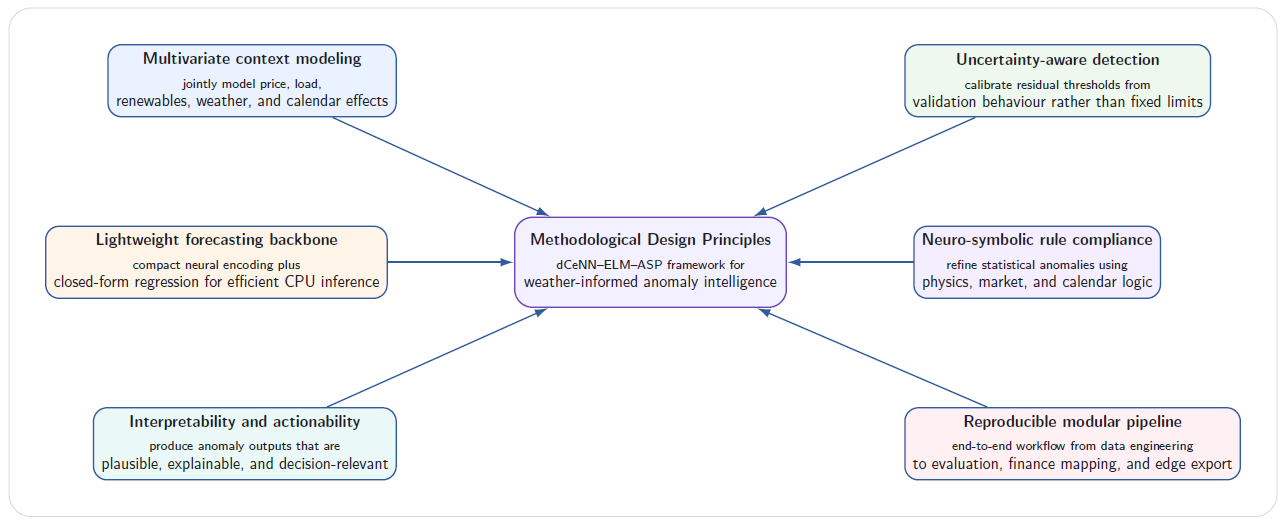
\includegraphics[width=\textwidth]{images/4.2.png}
	\caption{Methodological design principles guiding the proposed framework. The design combines
			efficient multivariate forecasting, uncertainty-aware residual analysis, symbolic rule-based
			refinement, and decision-oriented interpretation within a reproducible deployment-conscious pipeline.}
		\label{4.2}
	\end{figure}
	\FloatBarrier 

\subsection{Stage 1: Data Alignment and Feature Construction}

The first stage of the pipeline transforms heterogeneous raw sources into a single hourly feature table. According to the project description, the raw inputs consist of Austrian electricity-market and grid signals together with weather information and calendar context. In practice, the repository preprocessing step reads raw hourly power and price data, installed-capacity data, and weather variables, aligns them on a common UTC time index, and constructs the engineered dataset used throughout the rest of the workflow.

This stage is more than basic cleaning. It is the point where domain structure is introduced into the learning problem. The preprocessing script computes installed-capacity-aware solar and wind capacity factors, derives cyclical calendar encodings for hour, day-of-week, and month, constructs meteorological proxies such as air density, 100\,m wind speed, photovoltaic proxy terms, and wind power proxy terms, and adds Austrian public-holiday, weekend, and special-day indicators. The result is a feature space that contains both directly observed and physics-informed predictors, enabling the downstream model to learn how market and grid variables behave under changing exogenous conditions.

From a methodological perspective, this stage is essential because it defines what ``normality'' means for the neural forecaster. If the input representation omitted calendar and weather context, the model would confuse expected context-driven variation with abnormality. Thus, the first stage of the framework already contributes to anomaly quality by embedding explanatory context into the feature space.

\subsection{Stage 2: Leakage-Safe Split, Supervised Framing, and Scaling}

After feature construction, the pipeline converts the engineered hourly table into supervised learning matrices. The repository performs a strict chronological split into train, validation, and test periods and then creates lagged and rolling features over a selected core subset of variables. In the current implementation, these transformed inputs are saved to a compressed \texttt{NPZ} dataset that contains $X_{\text{train}}$, $X_{\text{val}}$, $X_{\text{test}}$, the corresponding multivariate targets, and metadata such as feature and target names. The fitted scaler is stored separately as \texttt{artifacts/scaler.npz} \cite{repo_split_scale}.

Formally, let $\mathbf{x}_t \in \mathbb{R}^{d}$ denote the engineered feature vector at time $t$, and let the multivariate target vector be
\begin{equation}
	\mathbf{y}_t =
	\begin{bmatrix}
		y_t^{(1)} & y_t^{(2)} & \cdots & y_t^{(m)}
	\end{bmatrix}^{\top},
	\label{eq:framework_targets}
\end{equation}
where, in the current implementation, the targets correspond to solar capacity factor, wind capacity factor, load, and electricity price. The supervised transformation augments $\mathbf{x}_t$ with lagged and rolling statistics:
\begin{equation}
	\tilde{\mathbf{x}}_t = \Phi\!\left(\mathbf{x}_t, \mathbf{x}_{t-1}, \dots, \mathbf{x}_{t-L}, \mathcal{R}_t\right),
	\label{eq:framework_supervised}
\end{equation}
where $\Phi(\cdot)$ denotes the feature-construction operator, $L$ is the lag horizon, and $\mathcal{R}_t$ denotes rolling summaries such as moving means. This enriched representation is then standardized using parameters estimated only from the training set.

This stage is methodologically central for two reasons. First, it creates the temporal memory available to the forecasting model without forcing the model itself to infer all temporal structure from raw inputs alone. Second, it prevents train--test contamination, which is crucial in anomaly detection because even subtle leakage can make residual-based methods appear stronger than they truly are.

\subsection{Stage 3: dCeNN Encoder as the Representation Layer}

The neural backbone of the framework begins with a lightweight discrete Cellular Neural Network encoder. Conceptually, the dCeNN maps the high-dimensional engineered input $\tilde{\mathbf{x}}_t$ into a compact latent state $\mathbf{h}_t$:
\begin{equation}
	\mathbf{h}_t = f_{\theta}\!\left(\tilde{\mathbf{x}}_t\right),
	\label{eq:framework_encoder}
\end{equation}
where $f_{\theta}(\cdot)$ denotes the dCeNN encoder. In the current implementation, this encoder is trained once and stored as \texttt{artifacts/dcenn\_encoder.pt}. The Tiny dCeNN temporal encoder that produces compact embeddings while keeping inference lightweight and CPU-friendly.

The role of the encoder in the overall methodology is to compress a large engineered feature space into a structured latent representation suitable for forecasting. Rather than passing the full input directly to a large recurrent or Transformer model, the framework deliberately uses a compact representation learner. This design decision supports both edge feasibility and methodological clarity: the encoder is the part of the pipeline responsible for learning a useful representation of normal context-conditioned system behaviour.

At the framework level, the most important point is not the exact implementation detail of each masked recurrent update, but the functional role of the dCeNN stage. It transforms raw engineered inputs into latent embeddings that summarize the relevant state of the grid--market system at time $t$ in a form that is easier to forecast and cheaper to deploy.

\subsection{Stage 4: ELM Ridge Head as the Forecasting Layer}

The encoded latent state is next passed to an Extreme Learning Machine style ridge-regression head. If $\mathbf{h}_t \in \mathbb{R}^{p}$ denotes the latent embedding, the forecast is produced as
\begin{equation}
	\hat{\mathbf{y}}_t = W^{\top}\mathbf{h}_t,
	\label{eq:framework_elm}
\end{equation}
where $W \in \mathbb{R}^{p \times m}$ is the output weight matrix estimated through a closed-form ridge solution \cite{huang2006extreme,hoerl1970ridge}. In matrix form, for latent design matrix $H$ and target matrix $Y$, the fitted weights are
\begin{equation}
	W = \left(H^{\top}H + \lambda I\right)^{-1}H^{\top}Y,
	\label{eq:framework_ridge}
\end{equation}
with ridge parameter $\lambda > 0$. The repository stores these learned regression heads in \texttt{artifacts/elm\_heads.npz}, alongside the target-name metadata.

Methodologically, the ELM head serves two purposes. First, it preserves training and inference efficiency: the prediction layer is solved analytically instead of being trained through long iterative optimization. Second, it keeps the model modular. The dCeNN learns the latent representation, while the ELM head defines the final multivariate forecast. This modularity is one of the reasons the framework is well suited to controlled experimentation, benchmarking, and eventual edge export.

The combination of dCeNN and ELM therefore yields a neural forecaster that is expressive enough to model multivariate normal behaviour, yet substantially lighter than many deep sequence baselines. In the overview of the pipeline, this stage corresponds to the main predictive ``brain'' of the framework.

\subsection{Stage 5: Residual Analysis and Statistical Anomaly Generation}

Once the multivariate forecast $\hat{\mathbf{y}}_t$ is available, the framework computes residuals as the primary statistical signal for anomaly generation:
\begin{equation}
	\mathbf{r}_t = \mathbf{y}_t - \hat{\mathbf{y}}_t.
	\label{eq:framework_residuals}
\end{equation}
For each target dimension $j$, the absolute residual $\lvert r_t^{(j)} \rvert$ is compared against a calibrated threshold $\tau_j(c_t)$ derived from the validation split:
\begin{equation}
	a_t^{(j)} = \mathbb{I}\!\left(\lvert r_t^{(j)} \rvert > \tau_j(c_t)\right),
	\label{eq:framework_flags}
\end{equation}
where $c_t$ denotes an optional context bucket such as hour-of-day or holiday state. The threshold-calibration stage is implemented separately from training, and the detection stage applies the resulting thresholds to the held-out test period to produce target-wise anomaly flags, threshold values, and a combined anomaly score.

The repository’s detection script makes this design explicit. It reloads the scaler, encoder, ELM heads, and thresholds, rebuilds the test supervised matrix, computes predictions and residuals, applies the selected bucketing strategy, and writes a full anomaly table to \texttt{reports/tables/anomalies\_2022.csv}. In addition to binary flags, the pipeline also computes a combined exceedance score:
\begin{equation}
	s_t = \sum_{j=1}^{m} \max\!\left(0,\frac{\lvert r_t^{(j)} \rvert}{\tau_j(c_t)+\varepsilon} - 1\right),
	\label{eq:framework_score}
\end{equation}
where $\varepsilon > 0$ is a small stabilizing constant. This score quantifies severity beyond the binary anomaly decision and provides a bridge to later event construction and downstream interpretation.

At the framework-overview level, this stage can be understood as the statistical anomaly generator. It converts forecast deviations into candidate anomalies. Importantly, however, these candidates are not yet treated as final decisions.

\subsection{Stage 6: ASP Veto as the Symbolic Refinement Layer}

The final stage covered by this overview is the ASP-based symbolic veto \cite{gelfond1988stable,gebser2019multi}. The motivation is straightforward: not every statistical residual exceedance should be accepted as a meaningful anomaly. Some flagged events may be physically implausible, contextually explainable, or economically irrelevant. The framework therefore introduces a symbolic reasoning stage that refines the statistical output before it is passed further downstream.

In implementation terms, the ASP script reads the anomaly table and the engineered feature table, converts selected quantities into symbolic facts, and invokes \texttt{clingo} over the rule base in \texttt{rules/market\_rules.lp} \cite{repo_detect_anomalies,repo_asp_apply,repo_market_rules}. The generated facts include anomaly indicators, holiday information, shortwave radiation, wind power, actual load, and a reference load baseline. The solver then returns two explicit categories:
\begin{itemize}
	\item \texttt{valid\_anomaly} atoms, representing anomaly candidates that survive the rule base;
	\item \texttt{vetoed} atoms, representing anomaly candidates rejected by symbolic logic.
\end{itemize}
The refined output is written to \texttt{reports/tables/anomalies\_refined.csv}.

Conceptually, this stage may be expressed as
\begin{equation}
	\tilde{a}_t^{(j)} = a_t^{(j)} \wedge \mathcal{R}\!\left(j,t,\mathbf{s}_t\right),
	\label{eq:framework_asp}
\end{equation}
where $a_t^{(j)}$ is the raw statistical anomaly flag, $\mathbf{s}_t$ is the context translated into symbolic facts, and $\mathcal{R}(\cdot)$ is the ASP reasoning process. The report describes this stage as a neuro-symbolic veto or repair layer that improves plausibility and interpretability by filtering false positives under domain constraints.

From the viewpoint of the overall methodology, this is the defining transition from purely statistical anomaly detection to neuro-symbolic anomaly refinement. The anomaly candidate has moved from a numerical object into a semantically constrained one. This is precisely what distinguishes the thesis framework from a conventional residual detector.

\subsection{Framework Summary and Stage-wise Traceability}

Table~\ref{tab:framework_overview_summary} summarizes the stage-wise logic of the pipeline and ties it to the implemented repository artifacts.

\begin{table}[H]
	\centering
	\caption{Stage-wise overview of the dCeNN--ELM--ASP pipeline.}
	\label{tab:framework_overview_summary}
	\small
	\begin{tabular}{|p{2.3cm}|p{3.2cm}|p{4.0cm}|p{6.1cm}|}
		\hline
		\textbf{Stage} & \textbf{Main operation} & \textbf{Purpose in the methodology} & \textbf{Representative implementation artifact} \\
		\hline
		Data preparation & Align raw market, grid, weather, and calendar data; compute engineered variables & Build a context-rich hourly feature space that supports conditional normality & \path{01_preprocess_build_features.py} \\
		\hline
		Split and scaling & Create lagged/rolling supervised matrices and apply train-only scaling & Enforce leakage-safe evaluation and standardized inputs & \path{02_split_and_scale.py}, \path{artifacts/scaler.npz} \\
		\hline
		dCeNN encoding & Map engineered inputs to compact latent embeddings & Learn a lightweight representation of normal multivariate behaviour & \path{artifacts/dcenn_encoder.pt} \\
		\hline
		ELM forecasting & Solve closed-form ridge regression in latent space & Produce fast multivariate forecasts with lightweight inference & \path{artifacts/elm_heads.npz} \\
		\hline
		Residual analysis & Compute residuals, calibrated thresholds, and anomaly scores & Generate statistical anomaly candidates under uncertainty-aware decision rules & \path{05_detect_anomalies.py}, \path{reports/tables/anomalies_2022.csv} \\
		\hline
		ASP veto & Convert anomaly outputs and context into facts and apply rule-based filtering & Reject implausible false positives and retain more interpretable anomalies & \path{07_apply_asp.py}, \path{rules/market_rules.lp}, \path{reports/tables/anomalies_refined.csv} \\
		\hline
	\end{tabular}
\end{table}

In summary, the framework overview reveals the essential methodological philosophy of the thesis. The pipeline begins with raw heterogeneous data, moves through representation learning and efficient multivariate forecasting, converts deviations into statistically grounded anomaly candidates, and finally subjects those candidates to symbolic reasoning before accepting them as refined anomalies. This staged structure is not incidental. It is the mechanism by which the thesis aims to combine efficiency, uncertainty awareness, interpretability, and rule consistency in a single anomaly-detection framework. The following sections deepen each of these components individually.


\section{The Neural Component}
\label{sec:neural_component}

The neural component of the proposed framework is responsible for learning a compact and context-aware model of normal multivariate grid--market behaviour. Its methodological role is not to classify anomalies directly, but to produce reliable forecasts of the expected target variables under prevailing operating conditions. Anomalies are then inferred from deviations between observed and predicted values in the next stage of the pipeline. This design choice is appropriate for the present thesis because large, clean anomaly labels are generally unavailable in electricity-market and grid data, whereas historical observations of mostly normal system behaviour are abundant.

Architecturally, the neural component is deliberately lightweight. It combines three tightly coupled elements:
\begin{enumerate}
	\item a feature-engineering and supervised-framing layer that transforms raw hourly observations into an informative multivariate input representation;
	\item a Tiny discrete Cellular Neural Network (dCeNN) encoder that compresses the engineered input into a compact latent embedding;
	\item an Extreme Learning Machine (ELM) style ridge-regression head that maps the latent embedding to multivariate forecasts in closed form.
\end{enumerate}
This structure is central to the thesis contribution. Instead of using a heavy end-to-end recurrent or Transformer model, the neural component separates representation learning from the final prediction layer. This yields a forecasting backbone that remains expressive, modular, and computationally economical.

\subsection{Design Objectives of the Neural Layer}

The neural layer is designed under four objectives.

First, it must be \emph{multivariate}. The system is intended to model joint behaviour across price, load, solar, wind, weather, and calendar context rather than treating each signal independently. This is essential because many meaningful anomalies in electricity systems are relationship anomalies, where the abnormality lies in inconsistent coupling among variables.

Second, it must be \emph{context-aware}. The model should not learn a single static baseline. It should learn how normal behaviour changes across time-of-day, season, weather conditions, and public-holiday status. The feature space therefore includes not only operational variables, but also exogenous and calendar covariates.

Third, it must be \emph{efficient}. The broader thesis explicitly values edge feasibility, CPU inference stability, and deployability. Consequently, the neural backbone is intentionally compact and avoids unnecessarily heavy iterative optimization in the forecasting head.

Fourth, it must be \emph{modular and reproducible}. The input transformation, encoder, and prediction head are separated into well-defined stages and artifacts. This makes the neural component easy to benchmark, inspect, and export.

\subsection{Feature Engineering and Supervised Representation}

The neural pipeline begins not with the encoder, but with the construction of a supervised multivariate feature representation. In the repository implementation, the preprocessing and split pipeline create an engineered hourly table from aligned market, grid, weather, installed-capacity, and calendar sources, then convert it into lagged and rolling supervised matrices for downstream training \cite{repo_preprocess_features,repo_split_scale}.

Let $\mathbf{x}_t \in \mathbb{R}^{d_0}$ denote the engineered base feature vector at time $t$. The base representation includes several feature groups:
\begin{itemize}
	\item \textbf{Operational variables:} actual load, solar generation, wind generation, and electricity price;
	\item \textbf{Meteorological variables:} temperature, relative humidity, wind speed, surface pressure, and shortwave radiation;
	\item \textbf{Derived physical proxies:} air density, 100\,m wind speed, wind-power proxy, and photovoltaic proxy;
	\item \textbf{Calendar encodings:} cyclic hour, day-of-week, and month representations;
	\item \textbf{Special-context indicators:} public-holiday, weekend, and special-day flags.
\end{itemize}

This engineered representation is then enriched with temporal memory. Specifically, the repository constructs lagged features and rolling means over a selected core subset of variables. The resulting supervised feature vector can be written as
\begin{equation}
	\tilde{\mathbf{x}}_t
	=
	\Phi\!\left(
	\mathbf{x}_t,
	\mathbf{x}_{t-1},
	\ldots,
	\mathbf{x}_{t-L},
	\mathcal{R}_t
	\right),
	\label{eq:neural_supervised}
\end{equation}
where $\Phi(\cdot)$ denotes the feature-construction operator, $L$ is the lag horizon, and $\mathcal{R}_t$ denotes rolling statistics such as moving means. In other words, the neural component does not receive a raw hourly vector; it receives a temporally enriched summary of the recent system state.

The multivariate target vector is
\begin{equation}
	\mathbf{y}_t
	=
	\begin{bmatrix}
		y_t^{(1)} &
		y_t^{(2)} &
		\cdots &
		y_t^{(m)}
	\end{bmatrix}^{\top},
	\label{eq:neural_targets}
\end{equation}
which in the current implementation corresponds to solar capacity factor, wind capacity factor, load, and price. The repository code exposes a horizon parameter in the supervised framing stage, while the present system primarily as a same-timestamp multivariate forecasting setup. The architecture is therefore best understood as \emph{horizon-ready}: its structure naturally supports shifted targets, even though the current thesis framing emphasizes the same-timestamp residual formulation \cite{repo_split_scale}.

From a methodological standpoint, this feature-engineering stage is critical. It embeds explanatory context directly into the neural input. Without weather and calendar information, the model would confuse expected context-driven variation with anomaly-generating deviation. Thus, feature engineering is not a peripheral preprocessing step; it is part of the anomaly-definition mechanism itself.

\begin{table}[htbp]
	\centering
	\caption{Feature groups used by the neural component.}
	\label{tab:neural_feature_groups}
	\small
	\begin{tabular}{|p{3.0cm}|p{6.0cm}|p{3.0cm}|}
		\hline
		\textbf{Feature group} & \textbf{Representative variables} & \textbf{Role in the model} \\
		\hline
		Operational signals & Load, solar MW, wind MW, price & Capture direct market and grid behaviour \\
		\hline
		Weather variables & Temperature, humidity, wind speed, pressure, shortwave radiation & Provide exogenous drivers of renewable and load variation \\
		\hline
		Derived proxies & Air density, 100\,m wind speed, wind-power proxy, PV proxy & Encode physically meaningful transformations of raw weather inputs \\
		\hline
		Calendar context & Hour/day/month cyclic encodings & Model periodic structure and seasonality \\
		\hline
		Special-day indicators & Holiday, weekend, special-day flags & Capture regime changes not explained by continuous variables alone \\
		\hline
		Lag and rolling features & Selected lags and rolling means over core variables & Provide short-term temporal memory in the supervised input \\
		\hline
	\end{tabular}
\end{table}

\subsection{The dCeNN Encoder as a Compact Representation Learner}

After feature engineering, the first trainable element in the neural pipeline is the dCeNN encoder. It can characterizes this module as a lightweight Tiny dCeNN temporal encoder, while the repository implements it as a compact masked recurrent encoder trained through an autoencoding objective \cite{repo_train_dcenn_elm}.

Conceptually, the encoder maps the supervised input $\tilde{\mathbf{x}}_t$ into a latent embedding $\mathbf{h}_t \in \mathbb{R}^{p}$:
\begin{equation}
	\mathbf{h}_t = f_{\theta}\!\left(\tilde{\mathbf{x}}_t\right),
	\label{eq:dcenn_map}
\end{equation}
where $f_{\theta}(\cdot)$ denotes the dCeNN encoder with parameters $\theta$.

The implementation follows a structured three-part design.

\paragraph{Input projection.}
The supervised feature vector is first projected into latent space:
\begin{equation}
	\mathbf{h}_t^{(0)} = \tanh\!\left(W_{\mathrm{in}}\tilde{\mathbf{x}}_t + \mathbf{b}_{\mathrm{in}}\right).
	\label{eq:dcenn_input_proj}
\end{equation}
This initial projection converts the high-dimensional engineered input into a lower-dimensional latent state.

\paragraph{Masked recurrent refinement.}
The latent state is then updated for a small number of recurrent steps using a block-structured connectivity mask:
\begin{equation}
	W_{\mathrm{eff}} = W_{\mathrm{cell}} \odot M,
	\label{eq:dcenn_weff}
\end{equation}
where $M$ is a binary block-diagonal mask and $\odot$ denotes element-wise multiplication. The recurrent update is
\begin{equation}
	\mathbf{h}_t^{(k+1)}
	=
	\tanh\!\left(
	W_{\mathrm{eff}}\mathbf{h}_t^{(k)} + \mathbf{b}_{\mathrm{cell}} + \gamma \mathbf{h}_t^{(k)}
	\right),
	\qquad k=0,\dots,K-1,
	\label{eq:dcenn_recurrence}
\end{equation}
where $\gamma$ is a residual mixing coefficient. In the actual training script, this coefficient is implemented as $0.3$, which provides stability-oriented residual mixing in each recurrent update \cite{repo_train_dcenn_elm}.

\paragraph{Latent embedding.}
After $K$ refinement steps, the final hidden state becomes the encoder output:
\begin{equation}
	\mathbf{H}_t = \mathbf{h}_t^{(K)}.
	\label{eq:dcenn_embedding}
\end{equation}

The dCeNN design is motivated by the theory of cellular neural computation, where local or structured connectivity is used instead of unrestricted dense recurrence \cite{chua1988cellular}. In the present implementation, locality is realized through the block-diagonal mask rather than through an explicit spatial lattice. This creates a structured latent transition matrix that is cheaper and more regularized than a fully connected recurrent matrix.

The current default encoder configuration is defined in \texttt{configs/dcenn.yaml}: latent dimension \texttt{enc\_dim = 48}, recurrent steps \texttt{steps = 2}, block size \texttt{block = 8}, autoencoder training epochs \texttt{ae\_epochs = 3}, learning rate \texttt{lr = 0.001}, weight decay \texttt{1e-4}, and seed \texttt{42} \cite{repo_dcenn_config}. The training script additionally defaults the mini-batch size to $256$ if it is not explicitly specified in the YAML configuration \cite{repo_train_dcenn_elm}.

\subsection{Why the Encoder Is Trained as an Autoencoder}

An important implementation detail is that the dCeNN encoder is not trained directly against the forecasting targets. Instead, the repository trains an autoencoder composed of the dCeNN encoder and a linear decoder, using the input reconstruction objective
\begin{equation}
	\mathcal{L}_{\mathrm{AE}}
	=
	\frac{1}{N}
	\sum_{t=1}^{N}
	\left\|
	\hat{\tilde{\mathbf{x}}}_t - \tilde{\mathbf{x}}_t
	\right\|_2^2.
	\label{eq:dcenn_autoencoder_loss}
\end{equation}
The rationale is methodological as well as practical. By training the encoder to reconstruct the standardized supervised input, the framework obtains a compact latent state that captures the dominant structure of normal operating conditions before fitting the final multivariate prediction head.

This is useful for three reasons. First, it decouples representation learning from the closed-form regression stage. Second, it keeps the encoder lightweight and stable. Third, it avoids the need for a fully backpropagated deep forecasting network, which would be more computationally expensive and less modular.

At the end of training, only the \emph{encoder} is exported; the decoder is discarded because it is not needed at inference time. This directly explains the role of the repository artifact \texttt{artifacts/dcenn\_encoder.pt}: it is the serialized \texttt{state\_dict} of the trained dCeNN encoder only, not of the full temporary autoencoder \cite{repo_train_dcenn_elm}. In other words, \texttt{dcenn\_encoder.pt} is the deployable representation-learning artifact of the neural component.

\subsection{The ELM Ridge Head as the Forecasting Layer}

Once the latent embeddings are available, the second trainable element of the neural component is the ELM-style forecasting head. Here, the term ``ELM'' is used in the broader sense of a fast analytical output layer rather than in the narrow sense of a fully random-hidden-layer classical ELM. In the present framework, the hidden representation is provided by the trained dCeNN encoder, and the output mapping is solved analytically as ridge regression \cite{huang2006extreme,hoerl1970ridge}.

Let
\begin{equation}
	H =
	\begin{bmatrix}
		\mathbf{H}_1^{\top} \\
		\mathbf{H}_2^{\top} \\
		\vdots \\
		\mathbf{H}_N^{\top}
	\end{bmatrix}
	\in \mathbb{R}^{N \times p},
	\qquad
	Y \in \mathbb{R}^{N \times m},
	\label{eq:elm_matrices}
\end{equation}
where $H$ is the latent design matrix and $Y$ stacks the multivariate targets. The forecasting head solves
\begin{equation}
	W = \left(H^{\top}H + \lambda I\right)^{-1}H^{\top}Y,
	\label{eq:elm_ridge_ch42}
\end{equation}
where $W \in \mathbb{R}^{p \times m}$ is the output weight matrix and $\lambda$ is the ridge regularization parameter. The final multivariate forecast is then
\begin{equation}
	\hat{Y} = HW,
	\qquad\text{or equivalently}\qquad
	\hat{\mathbf{y}}_t = W^{\top}\mathbf{H}_t.
	\label{eq:elm_prediction_ch42}
\end{equation}

The current default value of the ridge parameter is set in \texttt{configs/elm.yaml} as \texttt{l2 = 0.01} \cite{repo_elm_config}. This is methodologically attractive because it provides regularized closed-form fitting without iterative gradient descent. Training the head therefore reduces to solving one linear system rather than running an epoch-based optimization loop. That property is especially valuable for reproducibility and CPU-oriented deployment.

The corresponding deployable repository artifact is \texttt{artifacts/elm\_heads.npz}. According to the training script, this file stores two core elements:
\begin{itemize}
	\item the learned ridge-regression weight matrix $W$;
	\item the ordered list of target names associated with the output dimensions.
\end{itemize}
This means that \texttt{elm\_heads.npz} is the complete deployable forecasting head. During inference, the model only needs the encoder embedding $\mathbf{H}_t$ and this stored weight matrix to generate multivariate predictions \cite{repo_train_dcenn_elm}.

\subsection{End-to-End Neural Forward Path}

Taken together, the neural component performs the following sequence at inference time:
\begin{enumerate}
	\item transform the raw aligned hourly table into the engineered and supervised feature vector $\tilde{\mathbf{x}}_t$;
	\item standardize the feature vector using the training-fitted scaler;
	\item pass the standardized input through the exported dCeNN encoder from \texttt{dcenn\_encoder.pt};
	\item compute the multivariate forecast using the ridge weights stored in \texttt{elm\_heads.npz}.
\end{enumerate}
This can be written compactly as
\begin{equation}
	\hat{\mathbf{y}}_t
	=
	W^{\top}
	f_{\theta}\!\left(
	\mathrm{Scale}\!\left(\tilde{\mathbf{x}}_t\right)
	\right).
	\label{eq:neural_forward_path}
\end{equation}

The importance of this equation is methodological. It makes clear that the neural component is not an opaque monolith (reference from  the 2001: A Space Odyssey Sci-fi Novel and Film). It is a composition of a deterministic preprocessing path, an exported compact encoder, and an exported analytical prediction head. This decomposition improves traceability and supports the thesis objective of producing a reproducible and deployable anomaly-detection backbone.

\subsection{Why This Neural Design Is Appropriate for the Thesis}

The neural component reflects the broader engineering priorities of the thesis. The combination of engineered context, compact latent encoding, and closed-form regression offers a pragmatic balance between expressiveness and efficiency. It is more structured and domain-aware than a simple linear baseline, yet lighter than many deep recurrent or attention-based alternatives. This aligns with the literature on edge-oriented anomaly detection and lightweight model design, where local processing, modest memory footprints, and CPU-feasible inference are treated as central requirements rather than afterthoughts \cite{antonini2023tinyml,howard2017mobilenets}.

From a scientific perspective, the neural component also prepares the ground for the later symbolic stage in exactly the right way. It does not attempt to solve the entire anomaly problem on its own. Instead, it provides statistically informed and context-aware forecasts of normal behaviour. The resulting residuals then become the inputs to uncertainty-aware thresholding and, ultimately, to ASP-based refinement. In this sense, the neural component is the \emph{perception and prediction layer} of the overall neuro-symbolic framework: it estimates what the system should look like under normal conditions, while the symbolic layer decides whether deviations from that expectation should be accepted as meaningful anomalies.

\begin{table}[H]
	\centering
	\caption{Interpretation of the main neural artifacts in the repository.}
	\label{tab:neural_artifacts}
	\small
	\begin{tabular}{|p{4.0cm}|p{4.0cm}|p{6.0cm}|}
		\hline
		\textbf{Artifact} & \textbf{Stored content} & \textbf{Methodological role} \\
		\hline
		\path{artifacts/scaler.npz} & Training-fitted feature scaler & Ensures leakage-safe standardized inference matching the training distribution \\
		\hline
		\path{artifacts/dcenn_encoder.pt} & Exported \path{state_dict} of the trained dCeNN encoder & Provides the compact latent representation layer used during inference \\
		\hline
		\path{artifacts/elm_heads.npz} & Ridge weight matrix $W$ and target-name metadata & Implements the analytical multivariate forecasting head on top of latent embeddings \\
		\hline
	\end{tabular}
\end{table}

In summary, the neural component of the dCeNN--ELM--ASP framework is best understood as a carefully staged predictive module. Feature engineering injects context and temporal memory, the dCeNN encoder compresses the supervised input into a structured latent representation, and the ELM ridge head converts that representation into efficient multivariate forecasts. The exported artifacts \texttt{dcenn\_encoder.pt} and \texttt{elm\_heads.npz} are therefore not incidental implementation details; they are the deployable embodiment of the two main learnable parts of the neural pipeline. The next methodological stage takes the residuals produced by this neural component and subjects them to uncertainty-aware statistical testing and symbolic refinement.

\section{The Symbolic Component (ASP)}
\label{sec:symbolic_component_asp}

The symbolic component of the proposed framework is implemented through Answer Set Programming (ASP), which serves as the rule-aware reasoning layer of the overall neuro-symbolic pipeline. Its purpose is not to replace the neural forecaster, but to evaluate whether statistically flagged anomalies remain credible once domain constraints are taken into account. In the present thesis, the statistical detector produces candidate anomalies through residual exceedance, while the symbolic component acts as a structured filter, validator, and explanation mechanism. This stage is a \emph{neuro-symbolic veto/repair layer} that reduces false positives and improves plausibility, interpretability, and downstream utility.

This design is especially appropriate for electricity-market and grid data. Many statistical deviations are not operationally meaningful. A solar-related anomaly may be spurious if shortwave radiation is zero. A load deviation may be contextually explainable on a public holiday. A price anomaly may become more credible when supported by a simultaneous load anomaly. These cases illustrate a key methodological point: anomaly detection in energy systems is not only about measuring deviation, but also about interpreting deviation under rules, context, and domain constraints. ASP is used in this thesis precisely because it offers a declarative and non-monotonic formalism for that task \cite{gelfond1988stable,brewka2011asp,gebser2012answer,gebser2019multi}.

\subsection{Role of the Symbolic Layer in the Overall Framework}

At the system level, the symbolic component receives the outputs of the neural residual detector and transforms them from \emph{candidate anomalies} into \emph{rule-consistent anomalies}. If the neural stage produces a raw anomaly flag $a_t^{(j)}$ for target $j$ at time $t$, then the ASP layer applies a reasoning function $\mathcal{R}(\cdot)$ over symbolic facts and rules:
\begin{equation}
	\tilde{a}_t^{(j)} = a_t^{(j)} \wedge \mathcal{R}\!\left(j,t,\mathbf{s}_t\right),
	\label{eq:asp_refinement}
\end{equation}
where $\mathbf{s}_t$ denotes the symbolic context associated with the timestamp, such as holiday status, radiation level, wind generation, or load reference. The refined anomaly $\tilde{a}_t^{(j)}$ is therefore not merely a statistical exceedance; it is a statistical exceedance that also survives domain-level reasoning.

In the repository, this logic is implemented in \texttt{src/07\_apply\_asp.py}, which reads the anomaly table produced by the detection stage, generates symbolic facts from both the anomaly outputs and the engineered data, invokes \texttt{clingo}, and writes a refined anomaly table containing confirmed and vetoed cases \cite{repo_asp_apply}. The associated rule base is implemented in \texttt{rules/market\_rules.lp} \cite{repo_market_rules}. Although the user prompt refers to \texttt{07\_asp\_rules.lp}, the current repository operationalizes the same symbolic role through \texttt{market\_rules.lp}; this file is the actual ASP knowledge base used by the pipeline.

\subsection{Knowledge Engineering: From Domain Knowledge to Logic Rules}

A central methodological task in the symbolic component is \emph{knowledge engineering}: the process of translating domain knowledge into machine-executable logic. In this thesis, the goal of knowledge engineering is not to encode every conceivable energy-system rule. Instead, it is to encode a compact but meaningful subset of physical, calendar, and market consistency conditions that are directly relevant to anomaly filtering.

At a high level, the knowledge-engineering process follows four steps:
\begin{enumerate}
	\item identify domain regularities that should constrain anomaly interpretation;
	\item choose symbolic abstractions that capture those regularities;
	\item encode them as facts, rules, and constraints in ASP;
	\item use the resulting rule base to validate or veto statistical anomaly candidates.
\end{enumerate}

This process is inherently selective. Not every domain concept should be encoded symbolically. The symbolic layer is most useful for knowledge that is stable, trusted, interpretable, and difficult to guarantee through statistical learning alone. In the present framework, that includes:
\begin{itemize}
	\item \textbf{calendar regularities}, such as public-holiday exemptions;
	\item \textbf{physical plausibility conditions}, such as solar inconsistency at zero radiation;
	\item \textbf{temporal persistence logic}, which distinguishes noise from sustained events;
	\item \textbf{market sanity checks}, such as supporting some price anomalies through price--load co-anomaly confirmation.
\end{itemize}

It is important to be precise here. The current ASP rule base does \emph{not} implement a full market microstructure model, nor does it encode every possible market regulation such as explicit price-cap rules. Instead, the implemented rule base focuses on anomaly-plausibility filtering. In other words, it translates \emph{selected market and physical heuristics} into logic rather than attempting to formalize the entire electricity market. This is an advantage, not a weakness, because the rule base remains targeted, interpretable, and aligned with the anomaly-detection purpose of the thesis.

\subsection{ASP as the Formalism for Declarative Reasoning}

Answer Set Programming is a declarative paradigm in which knowledge is represented through facts, rules, and constraints, and reasoning is defined by stable-model semantics \cite{gelfond1988stable,gebser2012answer}. A generic ASP rule can be written as
\begin{equation}
	h \leftarrow b_1,\dots,b_m,\ \texttt{not}\ c_1,\dots,\texttt{not}\ c_n,
	\label{eq:asp_general_ch43}
\end{equation}
where $h$ is the rule head, $b_1,\dots,b_m$ are positive body literals, and \texttt{not} denotes default negation. The role of default negation is particularly important because it enables reasoning with exceptions and incomplete knowledge. This is one of the main reasons ASP is well suited to anomaly filtering in weather-driven energy systems.

For example, a candidate anomaly may usually be treated as valid, \emph{unless} it occurs on a public holiday, or \emph{unless} shortwave radiation is absent, or \emph{unless} wind variation exceeds a plausibility threshold. Such reasoning is inherently non-monotonic: adding a new fact may invalidate a previously acceptable conclusion. ASP handles this naturally, whereas simpler monotonic rule systems do not.

In the present thesis, ASP is used in a \emph{post-detection declarative reasoning} role. The neural component generates evidence from continuous multivariate data; the symbolic component evaluates that evidence using explicit rules. This makes the ASP layer a form of structured decision logic rather than a separate classifier.

\subsection{Fact Generation: Translating Continuous Data into Symbolic Atoms}

Because ASP operates on symbolic atoms rather than raw floating-point vectors, the first step in the symbolic component is to convert selected parts of the anomaly table and engineered data into facts. In the repository implementation, this happens in the helper function \texttt{\_generate\_facts(...)} inside \texttt{src/07\_apply\_asp.py} \cite{repo_asp_apply}. Each timestamp is first mapped to an integer hour index since the Unix epoch:
\begin{equation}
	t = \left\lfloor \frac{\mathrm{timestamp\_utc}}{3600} \right\rfloor,
	\label{eq:hour_index}
\end{equation}
which provides a solver-friendly discrete time representation.

The fact-generation process then emits four main categories of atoms.

\paragraph{1. Structural time facts.}
For every relevant time point, the script emits
\begin{equation}
	\texttt{hour}(t).
\end{equation}
This provides the symbolic system with an explicit time universe.

\paragraph{2. Statistical anomaly facts.}
For each target flagged by the neural detector, the script emits
\begin{equation}
	\texttt{anomaly}(\texttt{"target"}, t).
	\label{eq:anomaly_fact}
\end{equation}
These atoms are the neural-to-symbolic interface: they tell the rule base what the ML component currently believes is anomalous.

\paragraph{3. Calendar facts.}
If a timestamp corresponds to a public holiday, the script emits
\begin{equation}
	\texttt{holiday}(t).
	\label{eq:holiday_fact}
\end{equation}
This enables context-dependent reasoning, particularly holiday-based veto logic.

\paragraph{4. Physics and market observation facts.}
Selected engineered variables are discretized and emitted as atoms of the form
\begin{equation}
	\texttt{pred}(\texttt{signal}, v, t),
	\label{eq:pred_fact}
\end{equation}
where \texttt{signal} identifies the variable, $v$ is a rounded integer value, and $t$ is the hour index. The current implementation emits, among others:
\begin{itemize}
	\item \texttt{pred(shortwave\_radiation, V, t)}
	\item \texttt{pred(wind\_mw, V, t)}
	\item \texttt{pred(load\_mw, V, t)}
	\item \texttt{pred(load\_ref, R, t)}
\end{itemize}
The \texttt{load\_ref} signal is especially interesting because it is not a raw observation; it is a derived climatological reference constructed as the median load by hour-of-week. In other words, the fact-generation stage does not simply copy sensor values into logic. It also injects structured contextual references that the symbolic layer can reason over.

\begin{table}[H]
	\centering
	\caption{Main ASP fact families used in the symbolic component.}
	\label{tab:asp_fact_families}
	\small
	\begin{tabular}{|p{3.5cm}|p{5.5cm}|p{5.0cm}|}
		\hline
		\textbf{Fact family} & \textbf{Example atom} & \textbf{Purpose in reasoning} \\
		\hline
		Time facts & \path{hour(469512)} & Defines discrete solver time points \\
		\hline
		Neural anomaly facts & \path{anomaly("price", 469512)} & Encodes raw ML anomaly candidates \\
		\hline
		Calendar facts & \path{holiday(469512)} & Supports holiday-sensitive veto logic \\
		\hline
		Physics/market observations & \path{pred(shortwave_radiation, 0, 469512)} & Provides contextual evidence used by rules \\
		\hline
		Reference context facts & \path{pred(load_ref, 8450, 469512)} & Allows comparison against baseline operating conditions \\
		\hline
	\end{tabular}
\end{table}

\subsection{The ASP Rule Base: Logic Families and Their Meaning}

The current rule base in \texttt{rules/market\_rules.lp} is intentionally compact but methodologically rich \cite{repo_market_rules}. It defines five main rule families.

\paragraph{1. Persistence filter.}
The first rule family encodes the idea that isolated anomalies are less trustworthy than persistent ones:
\begin{align}
	\texttt{persistent}(G, T) \leftarrow
	&\ \texttt{anomaly}(G, T), \nonumber\\
	&\ \texttt{anomaly}(G, T-1), \nonumber\\
	&\ \texttt{anomaly}(G, T-2).
	\label{eq:persistence_rule}
\end{align}
This rule is a symbolic implementation of collective anomaly reasoning. It operationalizes the idea that meaningful disturbances often persist over short windows rather than appearing as single-timestamp noise spikes.

\paragraph{2. Physical plausibility constraints.}
The second family checks whether statistically flagged anomalies contradict simple physical logic. The implemented solar veto is
\begin{equation}
	\begin{aligned}
		\texttt{invalid\_solar}(T) \leftarrow & \ \texttt{anomaly("cf\_solar",T)}, \\
		& \ \texttt{pred(shortwave\_radiation,R,T)}, \\
		& \ R \le 0.
	\end{aligned}
	\label{eq:invalid_solar_rule}
\end{equation}
This rule expresses the intuitive principle that a solar anomaly is not operationally credible in the same way when there is no incident radiation. Similarly, the rule base defines a wind-ramp plausibility constraint:
\begin{align}
	\texttt{excessive\_wind\_ramp}(T) \leftarrow
	&\ \texttt{anomaly("cf\_wind",T)}, \nonumber\\
	&\ \texttt{pred(wind\_mw,V1,T)}, \nonumber\\
	&\ \texttt{pred(wind\_mw,V0,T-1)}, \nonumber\\
	&\ |V1 - V0| > \texttt{wind\_ramp\_limit}.
	\label{eq:wind_ramp_rule}
\end{align}
Here, the constant \texttt{wind\_ramp\_limit} is set to 500 in the rule file \cite{repo_market_rules}. This gives the rule base a concrete sanity bound.

\paragraph{3. Co-anomaly market logic.}
The third family captures a simple but important market-oriented relation:
\begin{equation}
	\texttt{confirmed\_economic\_spike}(T) \leftarrow
	\texttt{anomaly("price",T)},
	\texttt{anomaly("load\_mw",T)}.
	\label{eq:coanomaly_rule}
\end{equation}
This rule does not encode a full economic model, but it does introduce the idea that some price anomalies become more credible when supported by simultaneous load irregularity. This is a symbolic abstraction of cross-signal market consistency.

\paragraph{4. Final refinement logic.}
The core fusion rule of the symbolic layer is
\begin{align}
	\texttt{valid\_anomaly}(G,T) \leftarrow
	&\ \texttt{persistent}(G,T), \nonumber\\
	&\ \texttt{not holiday}(T), \nonumber\\
	&\ \texttt{not invalid\_solar}(T), \nonumber\\
	&\ \texttt{not excessive\_wind\_ramp}(T).
	\label{eq:valid_anomaly_rule}
\end{align}
This rule makes the overall philosophy of the ASP layer explicit. An anomaly is accepted not because the neural stage said so, but because it is persistent and does not violate the symbolic veto conditions. The rule base also includes a priority rule for price anomalies:
\begin{equation}
	\texttt{valid\_anomaly("price",T)} \leftarrow
	\texttt{confirmed\_economic\_spike}(T),
	\texttt{not holiday}(T).
	\label{eq:price_priority_rule}
\end{equation}
This means that co-anomalous price spikes can bypass the persistence requirement, which is a meaningful design choice: some market events may be important even if they are short-lived.

\paragraph{5. Explainability through veto tracking.}
The final rule family records not only which anomalies are rejected, but why:
\begin{align}
	\texttt{vetoed}(G,T) &\leftarrow \texttt{anomaly}(G,T), \nonumber \\
	&\quad \texttt{not valid\_anomaly}(G,T), \\
	\texttt{veto\_reason}(T,\texttt{"night\_solar"}) &\leftarrow \texttt{invalid\_solar}(T), \\
	\texttt{veto\_reason}(T,\texttt{"wind\_ramp\_limit"}) &\leftarrow \texttt{excessive\_wind\_ramp}(T), \\
	\texttt{veto\_reason}(T,\texttt{"holiday\_calendar"}) &\leftarrow \texttt{anomaly}(G,T), \texttt{holiday}(T).
	\label{eq:veto_reason_rules}
\end{align}
This is one of the strongest methodological aspects of the symbolic component. The ASP layer does not merely suppress anomalies; it produces a symbolic audit trail of the rejection logic.

\subsection{The Veto Mechanism as False-Positive Filtering}

The central operational function of the symbolic component is the \emph{veto mechanism}. The term veto is appropriate because the neural stage proposes anomaly candidates, but the ASP layer has the authority to reject them when they violate domain logic. The current implementation parses the ASP solver output into two lists:
\begin{itemize}
	\item a list of \texttt{valid\_anomaly(target, hour)} atoms;
	\item a list of \texttt{vetoed(target, hour)} atoms.
\end{itemize}
The final refined anomaly table then stores, for each retained or rejected item, the target, timestamp, hour index, anomaly score, final flag, and veto indicator \cite{repo_asp_apply}.

Methodologically, this veto mechanism addresses a specific weakness of purely statistical anomaly detection: the tendency to over-flag surprising points that are still physically plausible, contextually explainable, or economically trivial. This issue is identified as one of the main gaps in prior practice. The ASP stage is the thesis response to that gap. It reduces false positives not by tuning thresholds further, but by subjecting the flagged cases to domain-aware reasoning.

This logic is also evident in the repository’s small debugging script, which manually injects a ``solar anomaly at night'' fact together with zero radiation and tests the rule base through \texttt{clingo} \cite{repo_debug_clingo}. Although minimal, this script illustrates the exact spirit of the symbolic component: anomaly claims should be testable against explicit logic rather than accepted as opaque outputs.

\subsection{Interpretability, Modularity, and Limits of the ASP Layer}

The ASP layer adds three major strengths to the overall framework.

First, it improves \textbf{interpretability}. Because rules are explicit, users can inspect why an anomaly was accepted or rejected. The existence of named veto reasons further improves this transparency.

Second, it improves \textbf{modularity}. The symbolic layer can be updated without retraining the neural forecaster. If new domain knowledge becomes available, rules can be revised or expanded independently.

Third, it improves \textbf{trustworthiness}. A refined anomaly that survives rule-based scrutiny is more likely to be accepted by analysts than a raw black-box residual flag.

At the same time, the symbolic component has clear limitations, and a top-tier methodology section should state them openly. The current rule base is intentionally compact and therefore incomplete. It does not encode the full richness of market design, grid topology, or operational procedure. The symbolic layer also depends on the quality of fact generation: if continuous observations are discretized poorly or if important context is omitted, the rule base cannot compensate for that loss. Finally, symbolic rules are domain-dependent; transferring them to another market or grid context would require adaptation.

These limitations do not weaken the thesis contribution. Rather, they clarify its scope. The contribution of the symbolic component is not to solve every energy-reasoning problem, but to demonstrate how a compact and interpretable ASP layer can materially improve anomaly plausibility and explainability in a weather-driven grid--market anomaly pipeline.

\begin{table}[H]
	\centering
	\caption{Summary of the main ASP rule families in the current implementation.}
	\label{tab:asp_rule_families}
	\small
	\begin{tabular}{|p{3.5cm}|p{5.0cm}|p{6.0cm}|}
		\hline
		\textbf{Rule family} & \textbf{Representative logic} & \textbf{Methodological purpose} \\
		\hline
		Persistence rules & \path{persistent(G,T)} from 3-step support & Suppress isolated noise-like anomaly spikes \\
		\hline
		Physics-based veto rules & \path{invalid_solar(T)}, \path{excessive_wind_ramp(T)} & Reject anomalies that conflict with simple physical plausibility \\
		\hline
		Market logic rules & \path{confirmed_economic_spike(T)} & Confirm selected price anomalies through cross-signal consistency \\
		\hline
		Final fusion rules & \path{valid_anomaly(G,T)} & Produce the refined anomaly set used downstream \\
		\hline
		Explainability rules & \path{vetoed/2}, \path{veto_reason/2} & Record and categorize symbolic rejections for traceability \\
		\hline
	\end{tabular}
\end{table}

\subsection{Position of the Symbolic Component in the Thesis Methodology}

In the context of the full dCeNN--ELM--ASP framework, the symbolic component is the stage at which anomaly detection becomes \emph{domain-aware}. The neural component estimates what the multivariate system should look like under normal conditions. The statistical detector identifies where the observed system departs from that expectation. The ASP layer then decides which departures are worth preserving as refined anomalies once physical, calendar, and market logic are taken seriously.

This is the central methodological significance of the symbolic layer. It is not simply a rules appendix to a machine-learning model. It is the formal mechanism by which the thesis moves from black-box residual scoring toward interpretable, plausibility-aware, and operationally meaningful anomaly intelligence. The next section explains the hybrid integration point in more detail by showing how neural residuals and contextual variables are converted into ASP facts and how the two components interact programmatically.


\section{Hybrid Integration}
\label{sec:hybrid_integration}

The defining methodological contribution of the proposed framework lies not merely in the existence of both neural and symbolic components, but in the way they are integrated. The hybrid layer is the interface at which continuous multivariate predictions and residuals produced by the dCeNN--ELM forecaster are transformed into discrete symbolic evidence for Answer Set Programming. In other words, this stage explains how the pipeline moves from numerical anomaly scoring to rule-based anomaly validation. This transition is the movement from ML-generated anomaly candidates to an ASP-based \emph{repair/refinement layer} that confirms or suppresses those candidates using physical and market logic.

This integration point is central because the two subsystems operate over fundamentally different representations. The neural detector works in continuous Euclidean space. It consumes standardized lagged features, outputs multivariate forecasts, computes residuals, and applies calibrated thresholds. The ASP layer, by contrast, requires symbolic atoms such as \texttt{anomaly("price",t)} or \texttt{holiday(t)}. The hybrid integration stage is therefore not a trivial file conversion; it is a formal translation layer that preserves anomaly meaning while converting statistical evidence into a symbolic form that can be reasoned over declaratively.

\subsection{Why Hybrid Integration Is a Methodological Problem}

Neural anomaly detection and symbolic reasoning solve complementary but incompatible subproblems. The neural part is good at extracting regularities from noisy multivariate time series and defining a data-driven notion of normality. The symbolic part is good at enforcing explicit constraints, handling defaults and exceptions, and producing interpretable decisions. However, these two strengths do not combine automatically. A hybrid system must answer at least four methodological questions:
\begin{enumerate}
	\item Which numerical outputs from the neural model should be exposed to the symbolic reasoner?
	\item How should continuous values be discretized into logic facts without destroying their operational meaning?
	\item At what point in the pipeline should symbolic reasoning occur?
	\item What form should the final output take so that both confirmation and rejection are represented transparently?
\end{enumerate}

The present framework answers these questions in a particularly disciplined way. The ASP layer is applied \emph{after} residual thresholding, not before. Thus, the symbolic system does not receive all raw predictions and residuals as undifferentiated evidence. Instead, it receives a structured anomaly table already enriched with target-specific residual magnitudes, thresholds, binary anomaly flags, combined anomaly severity, and contextual metadata. This preserves the role of the neural stage as the statistical proposal generator while reserving the symbolic stage for plausibility-aware refinement.

\subsection{The Neural-to-Symbolic Interface in the Repository}

The repository implements the neural-to-symbolic handoff through a pair of consecutive scripts:
\begin{enumerate}
	\item \texttt{src/05\_detect\_anomalies.py}, which reconstructs the supervised test set, loads the trained neural artifacts, computes predictions and residuals, applies calibrated thresholds, and writes a full anomaly table \cite{repo_detect_anomalies};
	\item \texttt{src/07\_apply\_asp.py}, which reads that anomaly table together with the engineered feature table, converts selected values into facts, runs \texttt{clingo}, and writes the refined anomaly table \cite{repo_asp_apply}.
\end{enumerate}

This arrangement is methodologically clean because it makes the anomaly table the explicit interface object between the subsystems. The neural component does not call the ASP solver directly in-memory. Instead, it produces a reproducible artifact that can be inspected, audited, plotted, or reprocessed independently. This improves transparency and scientific traceability.

\subsection{Stage 1: Residual-Based Statistical Evidence from the Neural Component}

The first half of the hybrid integration is the construction of the neural anomaly table. In \texttt{src/05\_detect\_anomalies.py}, the trained encoder, ridge head, scaler, and threshold artifacts are reloaded, and the supervised test matrix is rebuilt from the engineered CSV using the same lag and rolling configuration used earlier in the pipeline \cite{repo_detect_anomalies}. The dCeNN encoder produces latent representations, the ELM head generates multivariate forecasts, and the detector computes residuals:
\begin{equation}
	\mathbf{r}_t = \mathbf{y}_t - \hat{\mathbf{y}}_t.
	\label{eq:hybrid_residual}
\end{equation}

For each target dimension $j$, the detector also computes absolute residuals and applies the calibrated threshold
\begin{equation}
	a_t^{(j)} = \mathbb{I}\!\left(\lvert r_t^{(j)} \rvert > \tau_j(c_t)\right),
	\label{eq:hybrid_target_flag}
\end{equation}
where $\tau_j(c_t)$ is derived from the threshold-calibration stage and may depend on a context bucket $c_t$. In the current configuration, the thresholding method is labeled \texttt{conformal}, with \texttt{alpha = 0.90} and \texttt{bucket\_by = hour}, meaning that the anomaly decision is calibrated against validation residuals and then bucketed by hour-of-day \cite{repo_thresholds_config}.

The anomaly table stores, for each target:
\begin{itemize}
	\item true value;
	\item predicted value;
	\item residual;
	\item absolute residual;
	\item threshold;
	\item binary anomaly flag.
\end{itemize}
It also stores three global summary quantities:
\begin{itemize}
	\item \texttt{combined\_score}, the summed normalized exceedance across targets;
	\item \texttt{n\_targets\_anom}, the number of targets anomalous at a timestamp;
	\item \texttt{any\_anomaly\_flag}, a binary indicator of whether any target is anomalous.
\end{itemize}

This structure is important for the hybrid system because it determines what statistical evidence is made available downstream. Rather than passing raw tensors or latent vectors into ASP, the framework passes a semantically meaningful anomaly table that is already interpretable in engineering terms.

\subsection{Stage 2: Symbolic Abstraction of Neural Outputs}

The second half of the integration is the conversion of neural outputs and engineered context into symbolic facts. Because ASP cannot reason directly over floating-point residual vectors, the framework performs an abstraction step in \texttt{src/07\_apply\_asp.py}. This abstraction does not simply discretize everything uniformly. It selectively exposes the information that is most useful for symbolic reasoning.

At the conceptual level, let $\mathcal{N}_t$ denote the set of neural outputs at time $t$ and let $\mathcal{C}_t$ denote the set of contextual engineered values. The fact-generation operator can be written abstractly as
\begin{equation}
	\mathcal{F}_t = \Gamma(\mathcal{N}_t,\mathcal{C}_t),
	\label{eq:fact_operator}
\end{equation}
where $\mathcal{F}_t$ is the symbolic fact set emitted for time $t$. In the implementation, $\mathcal{N}_t$ includes anomaly flags and anomaly score information, while $\mathcal{C}_t$ includes public-holiday status, radiation, wind power, actual load, and reference load.

This abstraction stage is a methodological compromise between two extremes:
\begin{itemize}
	\item passing too little information to ASP, which would make the symbolic layer weak and uninformed;
	\item passing too much low-level numerical detail, which would undermine the declarative clarity and efficiency of the rule base.
\end{itemize}
The repository chooses a compact middle ground: ASP receives target-level anomaly atoms and a small set of contextually meaningful explanatory variables.

\subsection{Stage 3: Time Normalization and Discrete Indexing}

One subtle but important part of hybrid integration is temporal normalization. The symbolic layer requires a discrete and solver-friendly representation of time. Accordingly, the ASP application script maps each UTC timestamp to an integer hour index:
\begin{equation}
	t = \left\lfloor \frac{\mathrm{timestamp\_utc}}{3600} \right\rfloor.
	\label{eq:hour_index_ch44}
\end{equation}
This serves two purposes. First, it makes temporal adjacency easy to express in ASP rules, as in $T-1$ and $T-2$ for persistence. Second, it avoids passing full datetime objects into the logical program, which would complicate grounding and solver operation.

This design decision is more important than it may initially appear. It is the reason the persistence rules and wind-ramp rules can be expressed in compact logical form. Without discrete time indexing, the symbolic layer would need a far more cumbersome temporal representation.

\subsection{Stage 4: Concrete Fact Families Produced by the Integration Layer}

The helper function \texttt{\_generate\_facts(...)} in \texttt{src/07\_apply\_asp.py} creates a string program of ASP facts from the anomaly table and engineered data \cite{repo_asp_apply}. Four main fact families are produced.

\paragraph{1. Time facts.}
Every relevant timestamp yields an atom of the form
\begin{equation}
	\texttt{hour}(t).
	\label{eq:hour_fact}
\end{equation}
This defines the symbolic time universe.

\paragraph{2. Neural anomaly facts.}
For every target flagged as anomalous by the statistical detector, the script emits
\begin{equation}
	\texttt{anomaly}(\texttt{"target"}, t).
	\label{eq:hybrid_anomaly_fact}
\end{equation}
A small but important implementation detail is that the script derives the ASP target names by scanning all columns that end in \texttt{\_anom} and mapping their display names to lowercase symbolic names. Thus, the neural target columns become the symbolic anomaly vocabulary.

\paragraph{3. Calendar facts.}
If the engineered data indicate a public holiday, the script emits
\begin{equation}
	\texttt{holiday}(t).
	\label{eq:hybrid_holiday_fact}
\end{equation}
This is the symbolic bridge between calendar-aware feature engineering and context-aware rule reasoning.

\paragraph{4. Context observation facts.}
Selected continuous observations are rounded and exposed as atoms of the form
\begin{equation}
	\texttt{pred}(\texttt{signal}, v, t).
	\label{eq:hybrid_pred_fact}
\end{equation}
The current implementation includes:
\begin{itemize}
	\item \texttt{pred(shortwave\_radiation, V, t)};
	\item \texttt{pred(wind\_mw, V, t)};
	\item \texttt{pred(load\_mw, V, t)};
	\item \texttt{pred(load\_ref, R, t)}.
\end{itemize}

The \texttt{load\_ref} fact is especially noteworthy because it is constructed inside the ASP application stage from a median load by hour-of-week, computed using the engineered data. This means that the hybrid layer does not merely forward upstream columns; it also derives symbolic reference context specifically for reasoning purposes.

Table~\ref{tab:hybrid_mapping_table} summarizes the mapping from neural/contextual data to ASP facts.

\begin{table}[H]
	\centering
	\caption{Hybrid mapping from neural outputs and engineered context to ASP facts.}
	\label{tab:hybrid_mapping_table}
	\small
	\begin{tabular}{|p{4.0cm}|p{5.0cm}|p{5.5cm}|}
		\hline
		\textbf{Source information} & \textbf{ASP form} & \textbf{Reasoning role} \\
		\hline
		Target anomaly flag from anomaly table & \path{anomaly("target", t)} & Encodes raw ML anomaly candidates \\
		\hline
		Timestamp & \path{hour(t)} & Supports discrete time reasoning and adjacency rules \\
		\hline
		Public-holiday indicator & \path{holiday(t)} & Enables holiday-sensitive veto logic \\
		\hline
		Shortwave radiation & \path{pred(shortwave_radiation, V, t)} & Supports solar plausibility checks \\
		\hline
		Wind generation & \path{pred(wind_mw, V, t)} & Supports wind-ramp plausibility checks \\
		\hline
		Actual load & \path{pred(load_mw, V, t)} & Supports market and context consistency logic \\
		\hline
		Derived load reference & \path{pred(load_ref, R, t)} & Provides baseline context for symbolic comparison \\
		\hline
	\end{tabular}
\end{table}

\subsection{Stage 5: Reasoning Fusion Through \texttt{clingo}}

Once the fact program has been built, the integration layer passes it to the ASP solver together with the rule base. In the repository, this occurs through \texttt{clingo.Control()}, followed by \texttt{add(...)} for the fact program, \texttt{load(...)} for the rule file, and \texttt{ground(...)} before solving \cite{repo_asp_apply}. Conceptually, the hybrid reasoning stage can be written as
\begin{equation}
	\mathcal{M}_t = \mathrm{ASP}\!\left(\mathcal{F}_t, \mathcal{K}\right),
	\label{eq:asp_model}
`v  \end{equation}
where $\mathcal{F}_t$ is the generated fact set and $\mathcal{K}$ is the rule base encoded in \texttt{market\_rules.lp}. The resulting stable model yields the symbolic outputs:
\begin{equation}
	\mathcal{O}_t = \{\texttt{valid\_anomaly},\ \texttt{vetoed},\ \texttt{veto\_reason}\}.
	\label{eq:asp_outputs}
\end{equation}

This is the precise point at which the neural and symbolic layers become one integrated system. The neural detector has already reduced the raw continuous sequence problem to a set of candidate irregularities. The symbolic layer then decides which of those irregularities are admissible under the encoded domain logic.

\subsection{Stage 6: Reconstructing Refined Anomalies as a Structured Output}

After solving, the repository parses the returned atoms into Python lists of valid and vetoed anomaly pairs. A time map from hour index back to UTC timestamp is then used to reconstruct a structured refined anomaly table. Each row in the resulting table contains:
\begin{itemize}
	\item the target identifier;
	\item the timestamp;
	\item the hour index;
	\item the anomaly score inherited from the neural anomaly table;
	\item \texttt{final\_flag}, indicating symbolic acceptance;
	\item \texttt{is\_vetoed}, indicating symbolic rejection.
\end{itemize}

This output design is methodologically strong for two reasons. First, it preserves the link to the original neural severity signal through the anomaly score. Second, it preserves the symbolic judgment explicitly rather than collapsing the refined output into a single opaque label. In other words, the hybrid layer does not overwrite the neural result; it annotates and restructures it through symbolic reasoning.

\subsection{Why the Integration Design Is Strong}

The hybrid integration strategy used in this thesis has four major strengths.

\paragraph{1. It is explicit.}
The interface between neural and symbolic components is visible as a real artifact: the anomaly table. This makes the system auditable and reproducible.

\paragraph{2. It is minimal but sufficient.}
Only selected facts are passed into ASP. The symbolic layer receives exactly the information needed for plausibility reasoning without becoming overloaded with irrelevant low-level detail.

\paragraph{3. It is modular.}
The neural detector can be changed without rewriting the symbolic rule base, provided the anomaly table schema remains stable. Likewise, rules can be revised without retraining the neural model.

\paragraph{4. It is interpretable.}
Because the translation from residuals to facts is explicit, one can trace the full path from continuous forecast deviation to symbolic anomaly decision.

\subsection{What the Integration Layer Does Not Do}

A rigorous methodology section should also state the limits of the current integration design.

First, the hybrid translation is \emph{selective rather than exhaustive}. Only a small subset of contextual variables is symbolized. Thus, the symbolic layer sees a curated view of the world, not the full neural state.

Second, the discretization of continuous values into rounded integers is a pragmatic design choice. It improves solver simplicity, but it inevitably loses some numerical precision.

Third, the current interface is primarily \emph{post-detection}. The symbolic layer does not influence neural training directly. It refines outputs after the statistical anomaly stage rather than co-training with it.

Fourth, the integration is designed for this specific Austrian market-grid anomaly use case. Its fact schema and rule vocabulary would need to be adapted for a different market, grid, or operational domain.

These limitations are acceptable in the context of the thesis because the goal of the hybrid layer is not to achieve perfect symbolic realism, but to create a principled bridge between residual-based anomaly detection and domain-aware anomaly validation.

\subsection{Methodological Significance of the Hybrid Layer}

The hybrid integration layer is where the thesis becomes genuinely neuro-symbolic. The dCeNN--ELM forecaster produces context-aware numerical expectations, the thresholding stage turns deviations into anomaly candidates, and the ASP layer then determines whether those candidates are compatible with simple but meaningful domain logic. The integration stage is the bridge that makes this cooperation possible.

Seen this way, the hybrid layer is not a minor implementation detail. It is the mechanism that converts a high-performing but purely statistical detector into a rule-aware anomaly-intelligence system. The neural component alone would produce anomalies that are numerically justified but not necessarily plausible. The symbolic component alone would lack the learned statistical sensitivity required to discover subtle multivariate deviations. The integration layer combines both strengths by translating residual-based evidence into symbolic facts that can be evaluated declaratively.

In summary, the hybrid component solves the representational mismatch between continuous residual analysis and discrete rule reasoning. It formalizes how anomaly evidence moves across that boundary, how context is preserved in symbolic form, and how final refined anomalies are reconstructed for downstream event analysis and utility-oriented interpretation. This makes it a core methodological contribution of the thesis rather than a mere engineering convenience.





